\documentclass[main.tex]{subfiles}

\begin{document}

\section{Design}
\label{Design}

\subsection{General Design Decisions}
We have chosen pandas dataframes \cite{pandas} as the common data format for both data exchange and any calculations. Pandas provides us with data structures ``that cohere with the rest of the scientific Python stack`` \cite{mckinney2011pandas}, such as NumPy, which we are using to calculate historical returns and risk metrics (\ref{BL Structure}). Additionally, it is supported natively by many third party APIs and can even be used to read data from SQL databases. For additional information, please consult the official pandas documentation \cite{pandas}.

\subsection{Overview of System Architecture}

Before discussing any specific component and architectural layer in depth, it is worth revisiting our original architecture \cite{TR}.
\begin{figure}[H]
	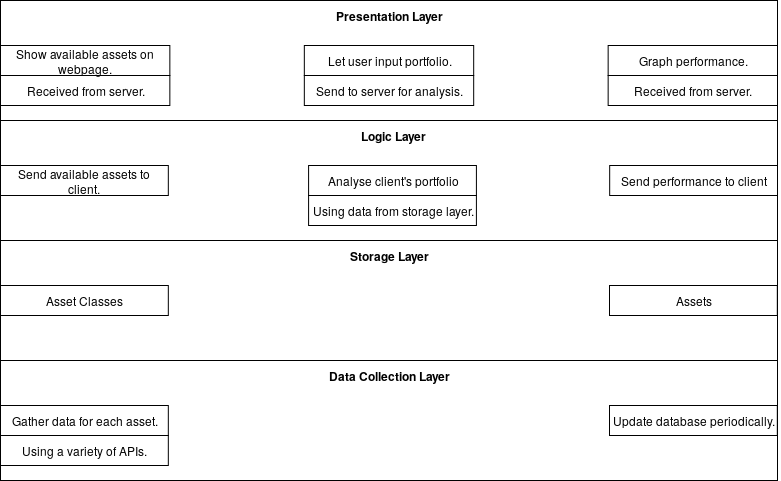
\includegraphics[width=\textwidth]{04Design/04Pictures/architecture_layer_diagram.png}
    \caption{Original Thalia System Architecture \cite{TR}}
\end{figure}
The above schematic illustrates how we modified a typical Three Layer architecture to include a Data Collection Layer. Subsequent discussion will refer to this layer as the `Data Harvester`. It consists of adapters for third party APIs which offer price data for financial assets. The associated API will be queried according to a configurable interval to allow for live updates to our price data. Additionally, initial seeding of the database with historical price data can also be achieved via the Data Harvester. The decision to isolate this system component has been made in order to increase security by limiting the access of the Thalia web service to the financial data database to read-only and to allow for independent scaling of the Data Harvester and our web service \cite{TR}.

While the architecture of our system has stayed the same, there have been some modifications to individual components. Most notable are the changes to the Database Structure examined in \ref{DB Structure}. The following sections will provide for a discussion of design decisions made on a layer-by-layer basis.

\subsection{GUI Structure}

The Graphical User Interface of Thalia consists of two main parts. One is a \emph{static} website created with HTML5 \cite{html5} and stylised with the help of Bulma \cite{bulma}. The second is a \emph{dynamic} Dash \cite{dash} page, which is basically the bulk of our application. In the following paragraphs we will discuss these separately. 

\subsubsection{Thalia Web}

Thalia Web consists of 5 pages, which all serve as an introduction to our application. We aimed at creating an authentic and modern looking website that attracts users. This was done by following a consistent style for the whole website, i.e. using the official colours, motto and Thalia logo, as discussed in \ref{Branding}.

While Thalia was not meant to be used on smaller devices due to the nature of our application, with the help of Bulma, every component of Thalia Web is responsive. Consequently, the layout of the website changes so that it fits the browser size perfectly.

Even though it is possible to navigate between pages by URLs directly, we have designed a navigation bar for this purpose. The look of this navigation bar depends on the device of the current user and whether the user has already been logged in or not. By default, an unauthenticated user will see the navigation bar visible on \figurename{\ref{thalia_navbar_design}}.

\begin{figure}[H]
   \centering
   
\includegraphics[width=\textwidth]{08Appendices/081User/081Pictures/navbar.png}
   \caption{Thalia Navigation Bar}
   \label{thalia_navbar_design}
\end{figure}

In case Thalia is launched on a mobile phone, the navigation bar becomes a so-called `hamburger button` and dropdown menu visible on \figurename{\ref{thalia_navbar_hamburger_design}}.

\begin{figure}[H]
   \centering
   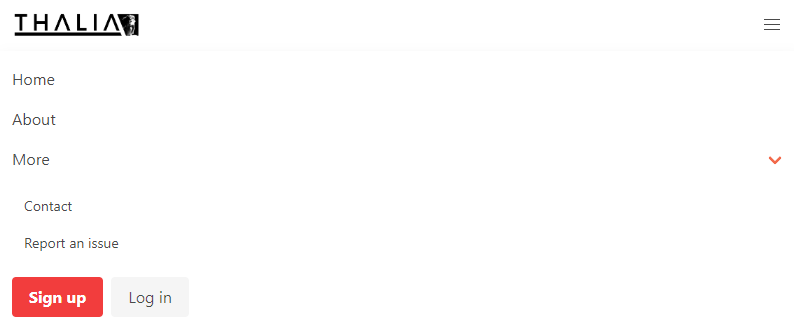
\includegraphics[width=\textwidth]{08Appendices/081User/081Pictures/navbar_hamburger.png}
   \caption{Thalia Navigation Bar - Hamburger}
   \label{thalia_navbar_hamburger_design}
\end{figure}

For the rest of this section we shall assume that the application was launched on a desktop, although the layout is identical and intuitive in the mobile case. 

\subsubsection*{Homepage}

We shall not discuss every page separately, as they are identical. For a full walkthrough, please refer to  \ref{user_manual}. As an example of our design choices, let us look at the homepage where users should arrive by default.

\begin{figure}[H]
   \centering
   
\includegraphics[width=\textwidth]{08Appendices/081User/081Pictures/homepage.png}
   \caption{Thalia Homepage (source: http://thaliabacktest.xyz/)}
   \label{thalia_home_design}
\end{figure}

As users arrive on the homepage, they are greeted with a short description of Thalia and the process of backtesting. We have designed the homepage such that the navigation bar and the Thalia Logo fills the screen completely. To indicate that the page does not end there, we have added a scroll down button, which with the help of a JavaScript \cite{js} animation takes the user down to the bottom of the page. Here, the user may encounter a small register form, or in case the user is logged in, a link to the dashboard, i.e. the main application.

\begin{figure}[H]
   \centering
   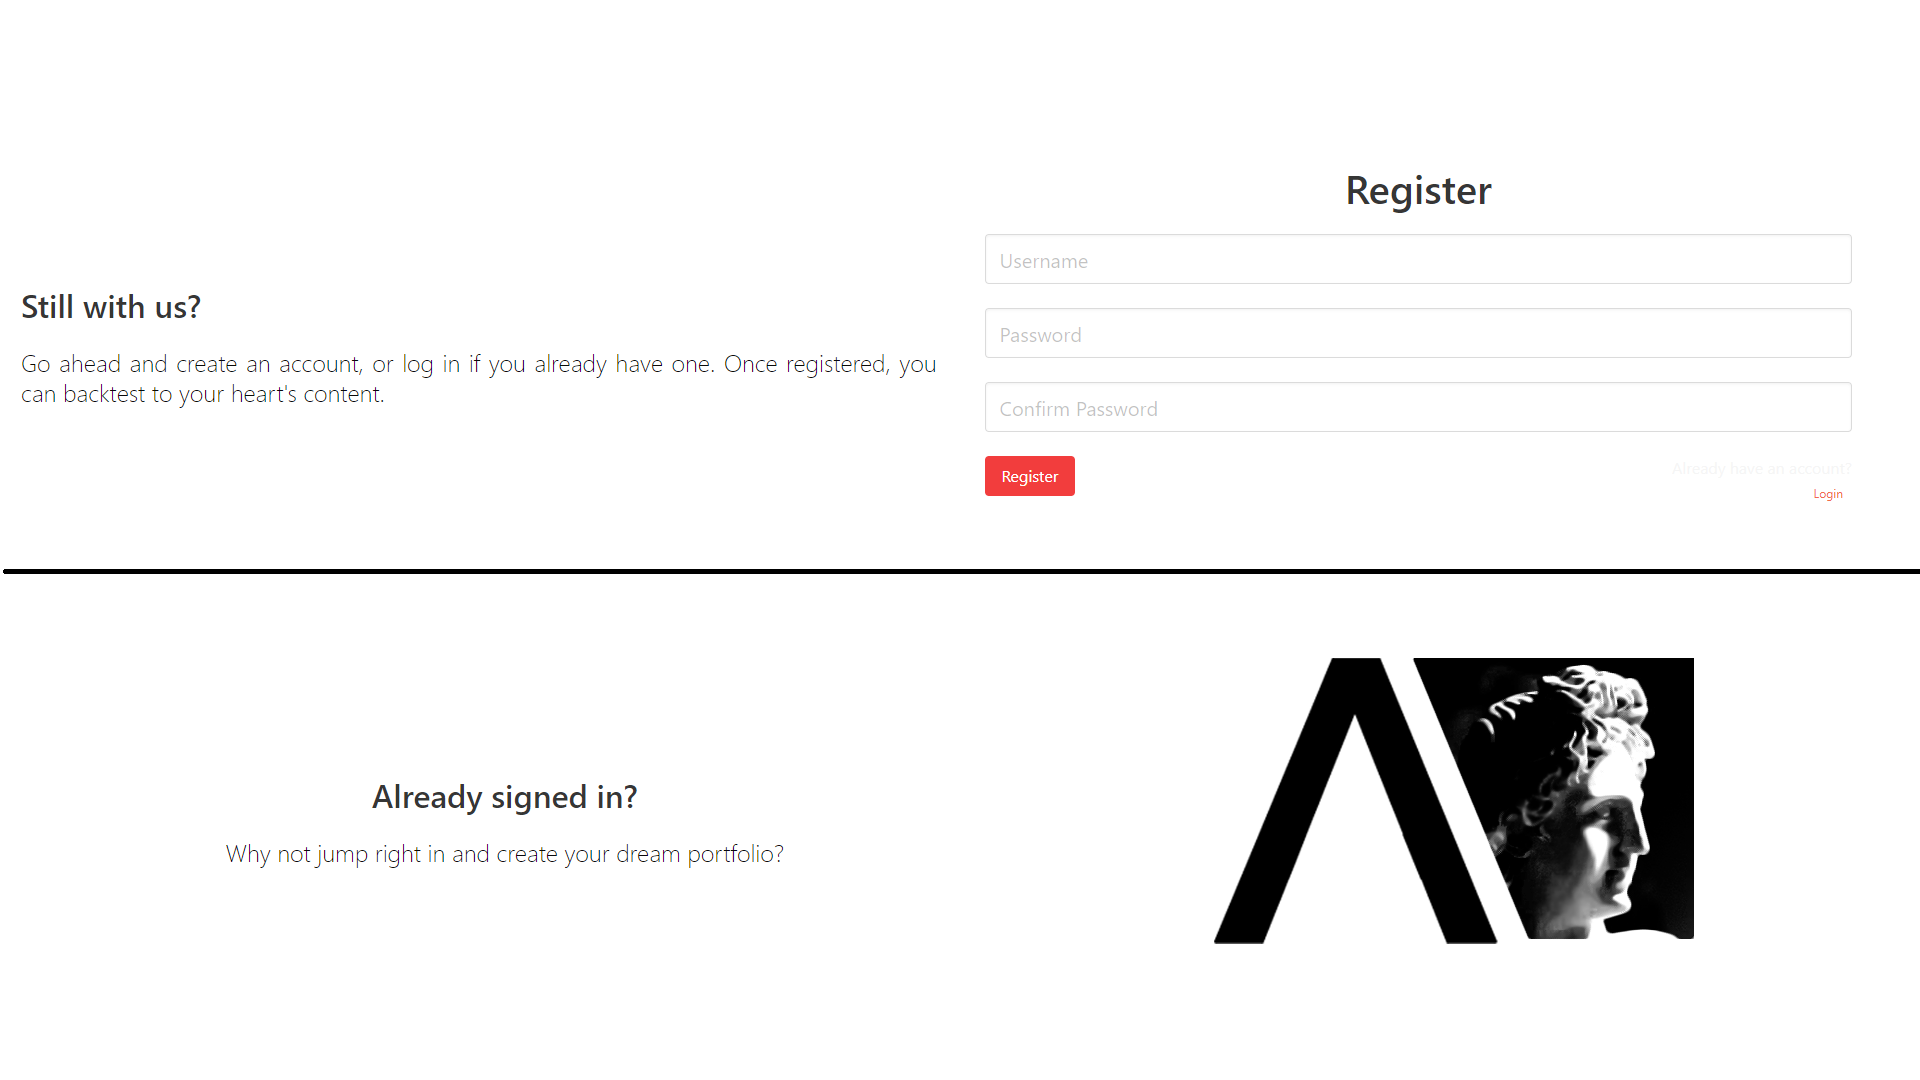
\includegraphics[width=\textwidth]{08Appendices/081User/081Pictures/homepage_bottom.png}
   \caption{Top: User not logged in; Bottom: User recognised}
   \label{thalia_home_bottom_design}
\end{figure}

\subsubsection*{Log In and Sign Up Pages}

In case the user is not yet logged in, links for the `Log In` and `Sign Up` pages are visible on the navigation bar as seen on \figurename{\ref{thalia_navbar_design}} or \figurename{\ref{thalia_navbar_hamburger_design}}.
Both of these forms are quite common, with the login requiring:

\begin{itemize}
    \item Username
    \item Password
    \item (Optional) Remember me
\end{itemize}

And for signing up, the fields are:

\begin{itemize}
    \item Username
    \item Password
    \item Confirm Password
\end{itemize}

As standard, the registration fails when the user enters different values to the `Password` and `Confirm Password` fields. In this case, the user is prompted to try again.

\begin{figure}[H]
   \centering
   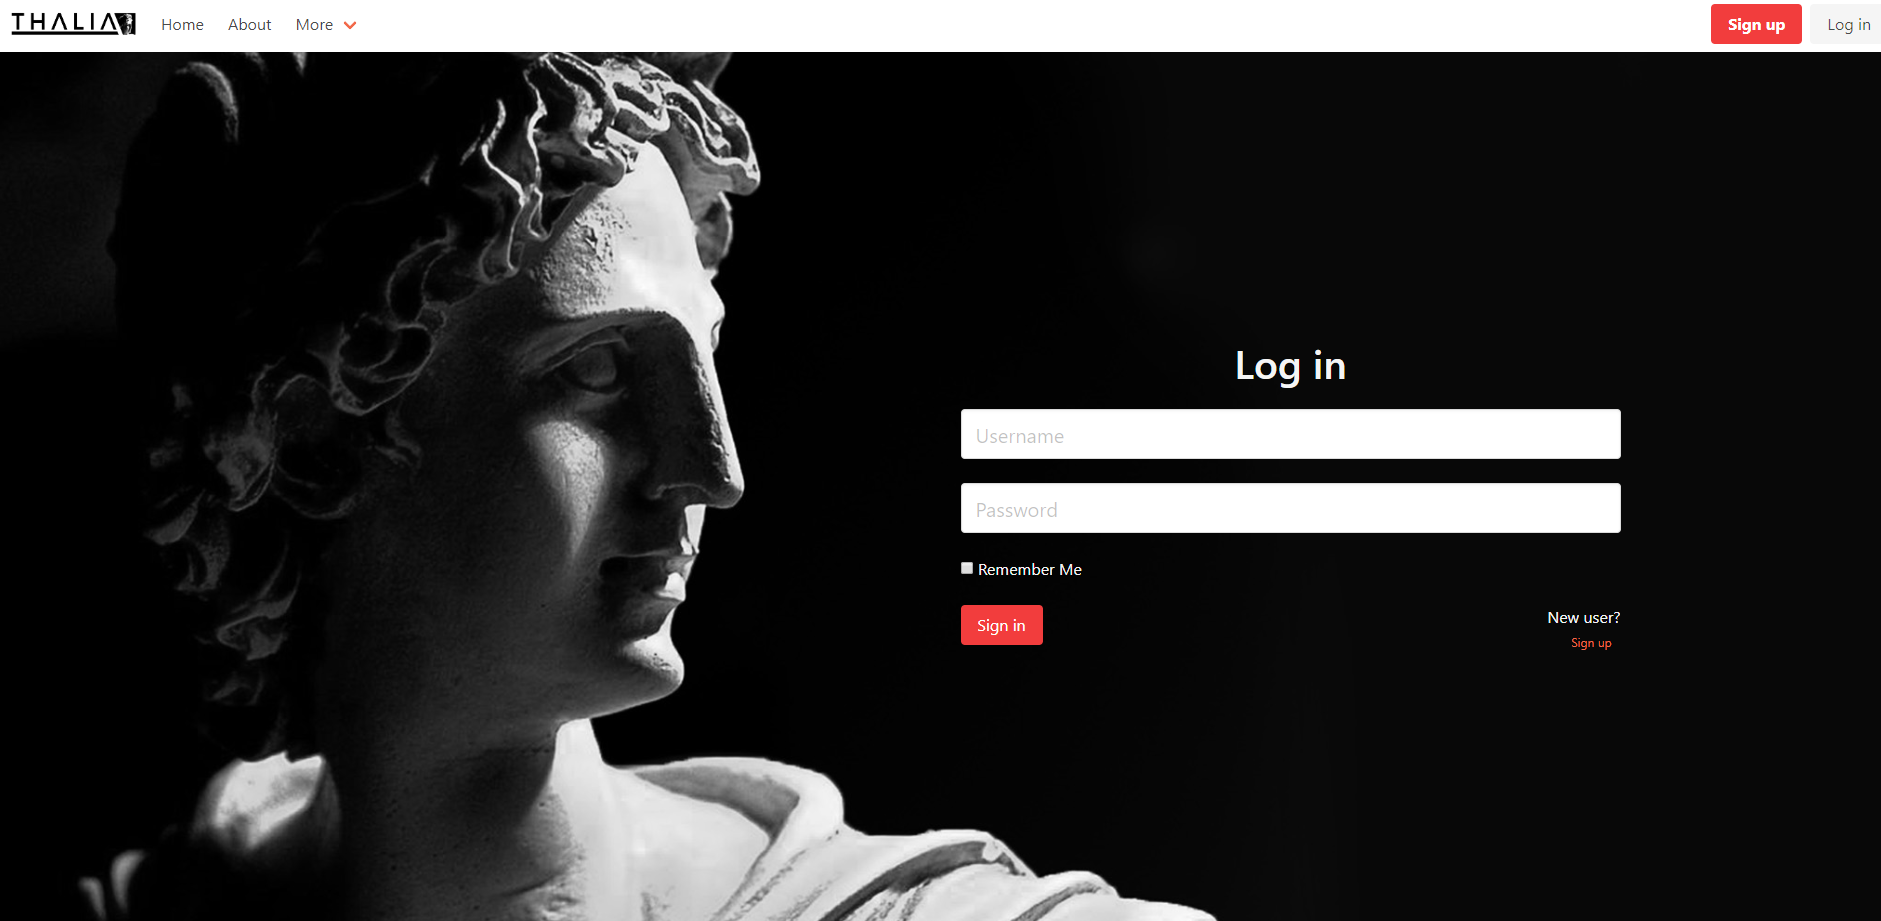
\includegraphics[width=\textwidth]{08Appendices/081User/081Pictures/login.png}
   \caption{Thalia Log In Page (source: http://thaliabacktest.xyz)}
   \label{thalia_login_design}
\end{figure}

In case the user is already logged in and attempts to access these pages, they will be redirected to the homepage. Additionally, the navigation bar changes, allowing us to log out.

\subsubsection{The Dashboard}

\say{Dash apps are composed of two parts. The first part is the `layout` of the app and it describes what the application looks like. The second part describes the interactivity of the application [...]} \cite{dash_layout}. Creating the Dashboard with Dash meant using Python classes for all of the visual components of the application.

Writing code for the layout was intuitive, but cumbersome, as on top of the HTML-like structure, it also needed to be correctly indented. Consequently, we needed to rely on refactoring a lot, chopping the layout code into smaller, more manageable components. In our final design, we have decided to divide the Dashboard into tabs, which helped us achieve a more intuitive look and organised codebase. The layout of the dashboard can now be initialised as follows:

\begin{lstlisting}[language=Python, caption=layout.py - Example of Dash Code, label=lst:dash_code]
import dash_core_components as dcc
import dash_html_components as html
from . import tabs

layout = html.Div(
    html.Main(
        [
            html.Div(
                [
                    dcc.Tabs(
                        [
                            tabs.tickers(),
                            tabs.summary(),
                            tabs.metrics(),
                            tabs.returns(),
                            tabs.drawdowns(),
                            tabs.assets(),
                        ],
                        id="tabs",
                        value="tickers",
                    ),
                ],
                className="column",
            ),
        ],
        className="columns",
    ),
    className="section",
)
\end{lstlisting}

Upon arriving at the Dashboard, only the `Ticker Selection` tab is available to the user. This is where the user is expected to input their investment strategy. Although this process is fairly intuitive and done by using dropdown menus, input fields and standard date selectors, a more thorough walkthrough can be found in \ref{user_manual}. 

For the selection of assets we have decided to take an alternative approach visible on \figurename{\ref{thalia_table_design}}. This was done mostly because of the limitations of Dash discussed in \ref{dash_limitations}, but came with its own benefits.

\begin{figure}[H]
   \centering
   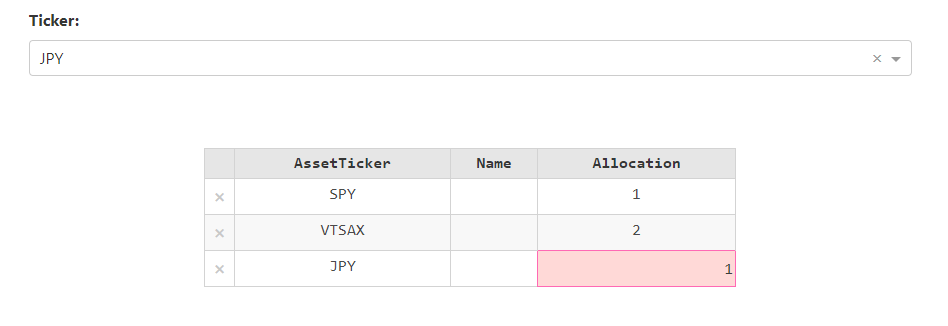
\includegraphics[width=\textwidth]{08Appendices/081User/081Pictures/table.png}
   \caption{Thalia Dashboard - Assets Table}
   \label{thalia_table_design}
\end{figure}

The official documentation describes the dash table as \say{an interactive table component designed for viewing, editing, and exploring large datasets} \cite{dash_table}. Working with the dash table is also quite simple, as its data can be accessed by addressing the id of the table and then the data component. For a further explanation on registering Dash Components, read \ref{GUI}.

Accessing the data like this also allowed us to fulfill one of our requirements, which is to support portfolios with a large number of assets. This would have been significantly harder, if not impossible, with alternative approaches, see \ref{dash_limitations}.

To compare investment strategies, the user may add portfolios via the `Add Portfolio` button. Due to the arguments presented in \ref{dash_limitations}, we have decided to set the maximum number of portfolios to 5, compared to letting it be dynamic. In addition, it is possible to select from a set of benchmarks, also known as lazy portfolios. Having selected one, the user will find the table populated with the desired assets and proportions. 

When the user is content with the input, they can start backtesting by clicking the `Submit` button. If all required fields are populated, the user is taken to the summary tab. This, as well as all other tabs, is now unlocked.

\subsubsection*{Showing the Results}

Many studies have shown that one most important factor when designing a dashboard application is to show the right data using the right visualization tools \cite{dashboard_design1} \cite{dashboard_design2}. In our case, we have already established which metrics and plots are most important to the users. When the user lands on the summary tab, it is these key metrics that are presented, leaving a more detailed analysis for the relevant tabs. This way the user is not overloaded with information as soon as the results are presented. 

Having decided on `What` the user should see we can now focus on the `How`. In our final design, we combine data visualization techniques to make the dashboard look interesting. Key metrics are shown either in a `box`, which is a core building block of a dashboard or in tables. Proportions are visualised using pie charts, whereas relative differences are shown with the help of a bar chart. Some examples can be seen on \figurename{\ref{dashboard}}.

\begin{figure}[H]
   \centering
   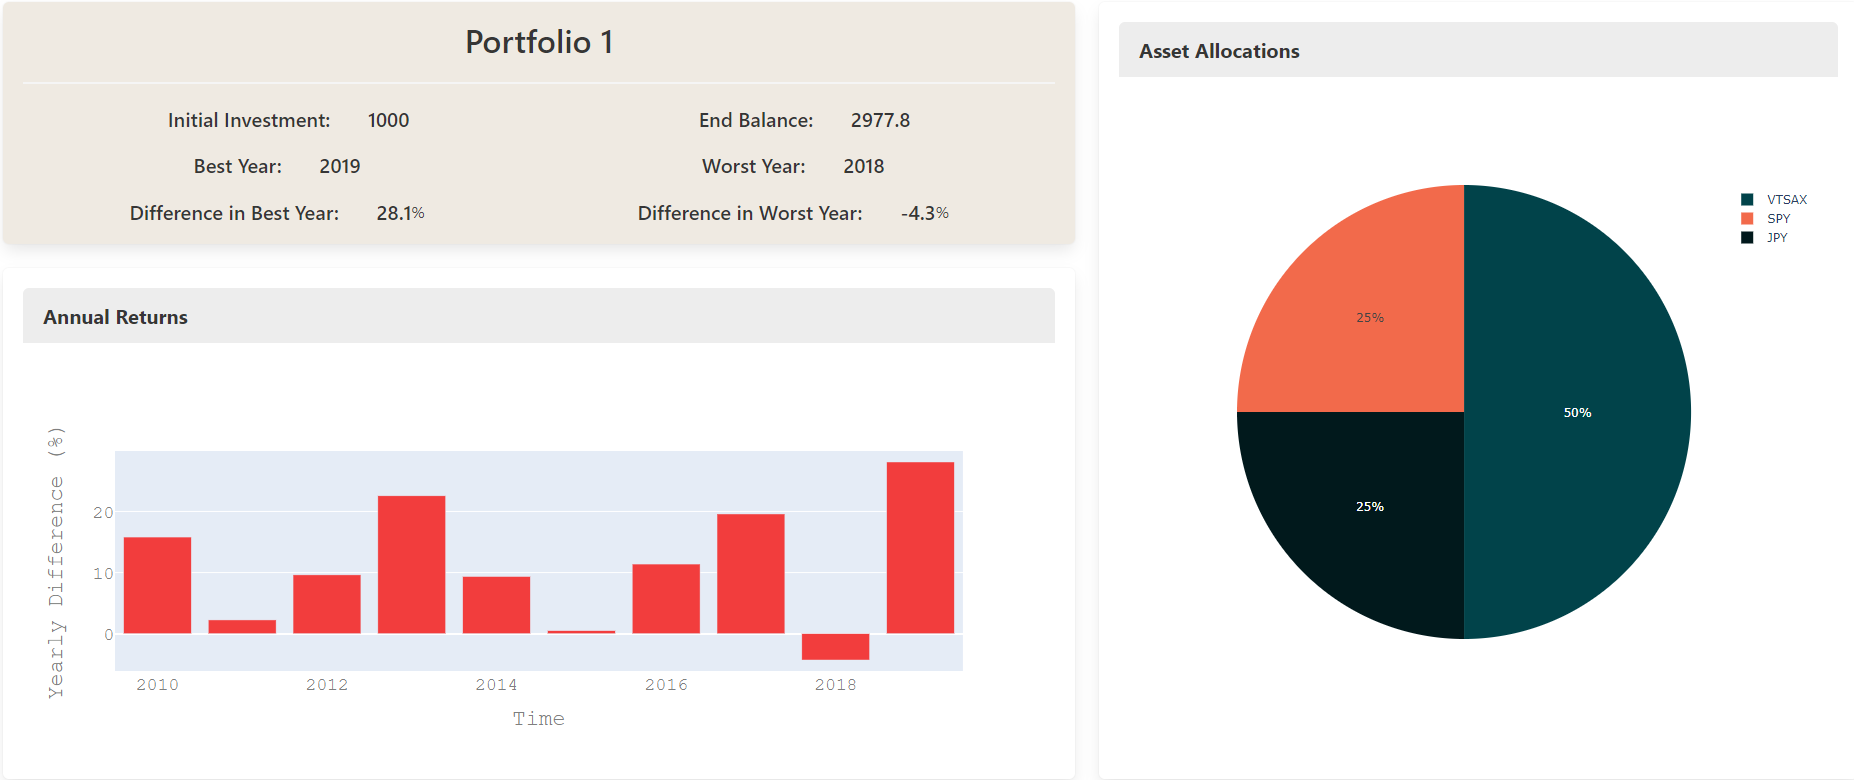
\includegraphics[width=\textwidth]{04Design/04Pictures/dashboard.png}
   \caption{The Dashboard}
   \label{dashboard}
\end{figure}

Among these charts, the user can find one of the key components of our application, the Portfolio Growth Plot. This graph is crucial for our application, as it serves as a visualisation for two of our main functional requirements, i.e. showing the total returns of a portfolio over time and the comparison of strategies.
Thanks to Dash, all graphs are fully interactive. The user may zoom in on selected areas, hover over desired data points, save the plot as an image, etc.

\begin{figure}[H]
   \centering
   
\includegraphics[width=\textwidth]{08Appendices/081User/081Pictures/dash_funcionalities.png}
   \caption{Dash Functionalities}
   \label{dash_functionalities_design}
\end{figure}

The result of performing one such action on the Portfolio Growth Plot can be seen on \figurename{\ref{portfolio_growth}}. In this case, the user is about to enlarge the selected region to inspect the plot closer. Resetting the graph can then be done by one of the buttons visible on \figurename{\ref{dash_functionalities_design}}.

\begin{figure}[H]
   \centering
   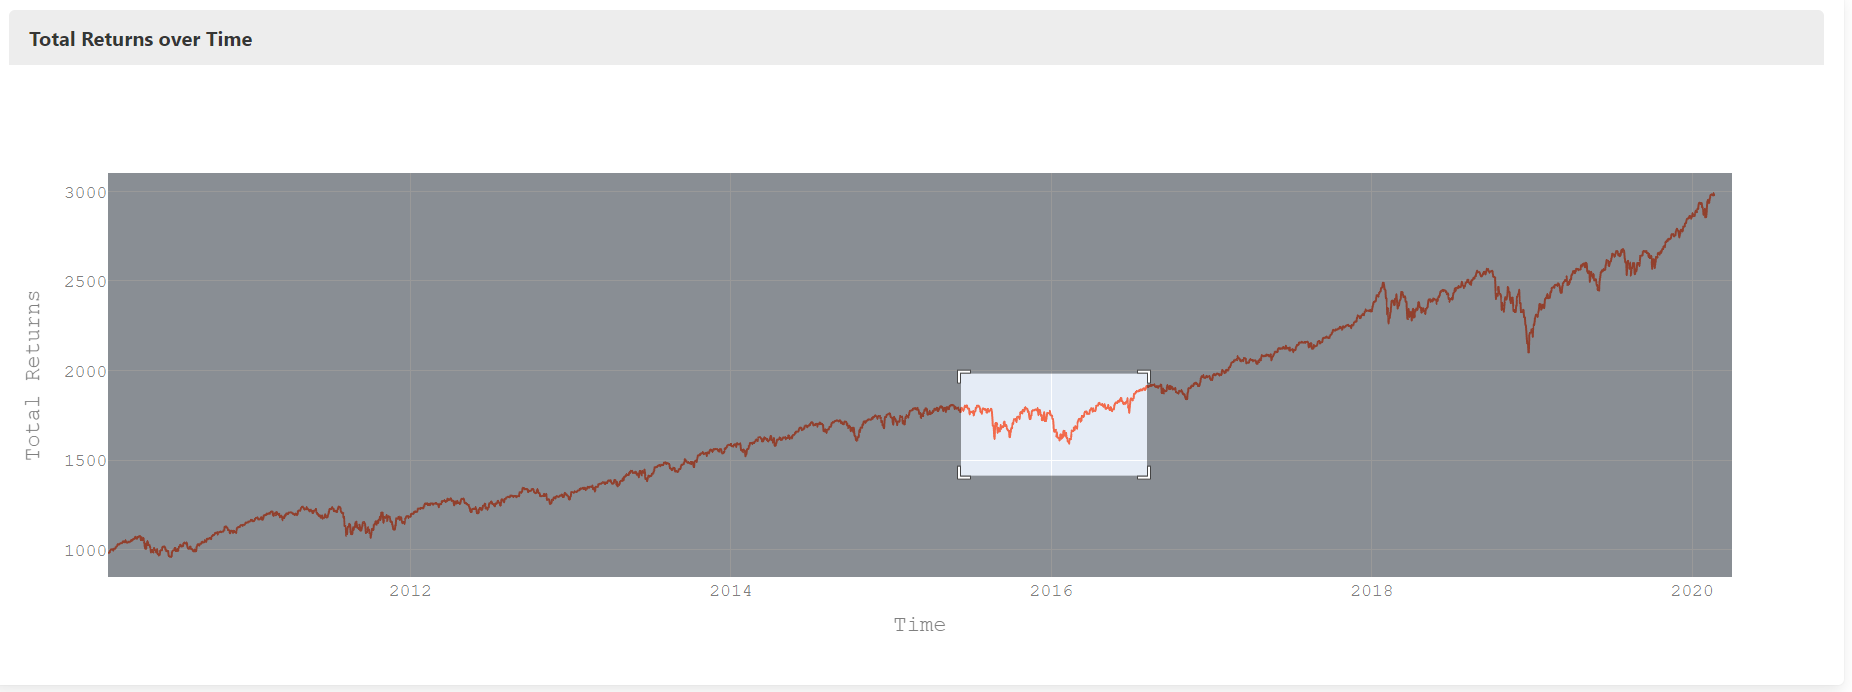
\includegraphics[width=\textwidth]{04Design/04Pictures/portfolio_growth.png}
   \caption{Dash Functionalities - Portfolio Growth}
   \label{portfolio_growth}
\end{figure}

\subsubsection{Changes to the Initial Design}

The design of the Dashboard was done according to the wireframes we have provided last term \cite{TR}, also visible on \figurename{\ref{wireframe}}.

\begin{figure}[H]
   \centering
   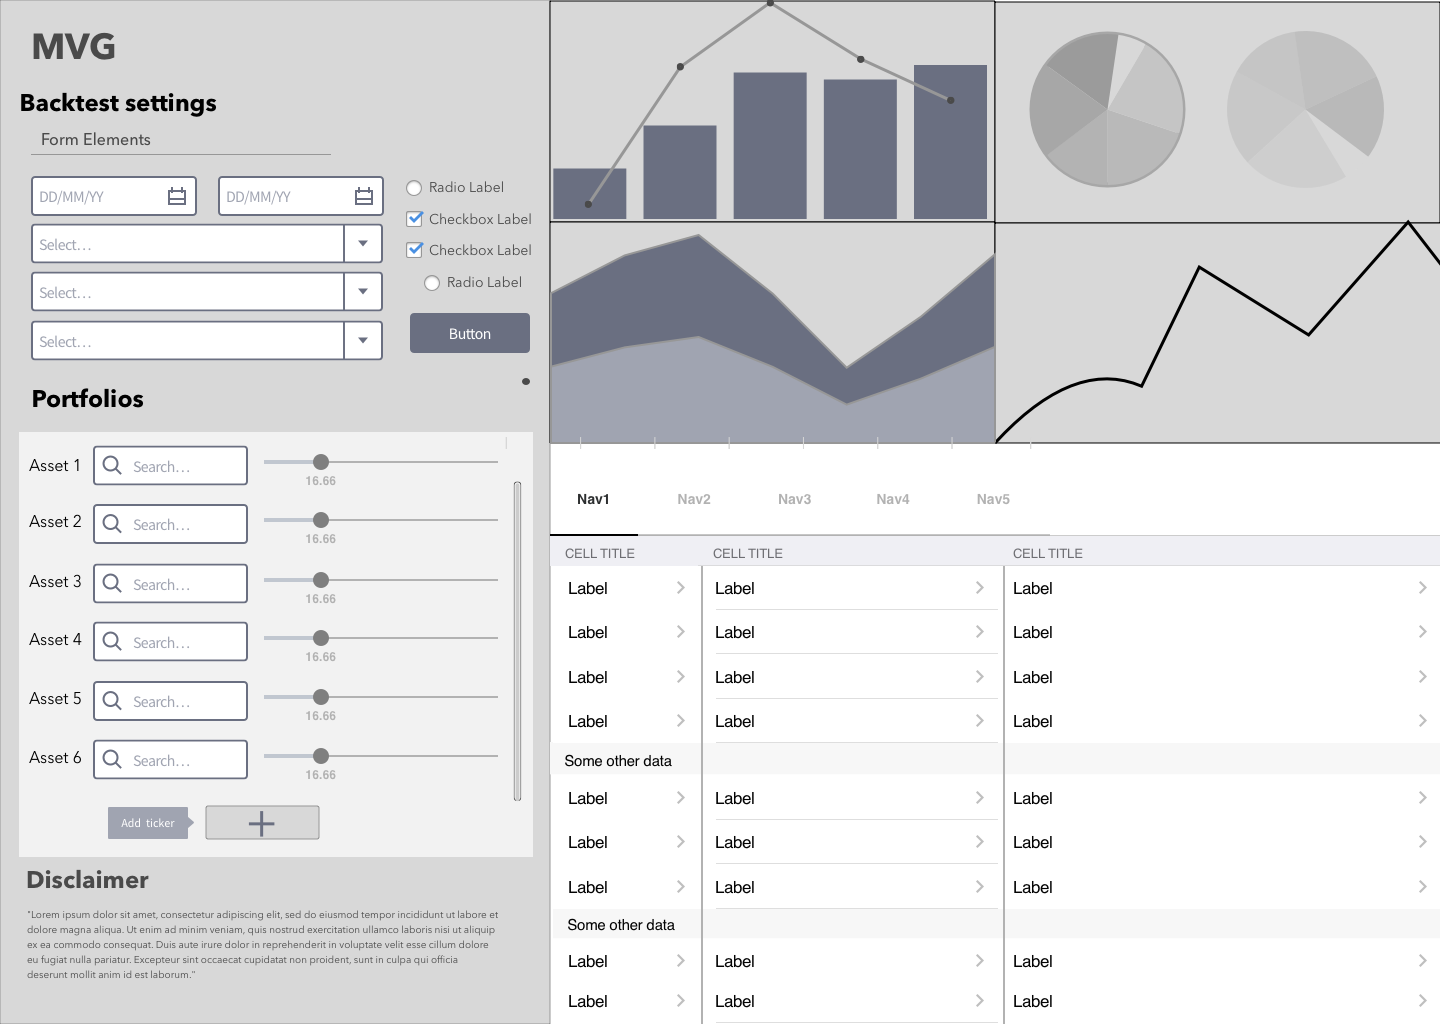
\includegraphics[width=\textwidth]{04Design/04Pictures/wireframe.png}
   \caption{UI Wireframes}
   \label{wireframe}
\end{figure}

As we can see, we managed to encapture the overall look as we envisioned with only minor changes. The data is significantly better distributed by the use of tabs, giving a less cluttered UI. Additionally, we have decided not to implement the aside menu, partly because it was unnecessary, but mostly because it suggests that the backtest results can be changed on the go. This, as we have realised, was not feasible, due to expensive calculations in the Business Logic Layer.

One change we had to make was the use of the Dash table instead of the approach visible on \figurename{\ref{wireframe}}. The benefits of this change have been illustrated further above. In addition, we have also decided to discard the sliders as a way of changing asset allocations.

For portfolio comparison, we also had to enable inputting multiple strategies. As seen on \figurename{\ref{wireframe}}, this is something we have not accounted for when planning the design. The implementation of this feature led to a full refactoring of the UI code, as it came with an excessive amount of code due to the arguments presented in \ref{dash_limitations}. Fortunately, this issue was addressed relatively early and resulted in the current design. 

\subsection{Business Logic Structure}
\label{BL Structure}

The responsibility of our business logic can be summarised as follows: Given an investment strategy specification input from a user via the GUI, retrieve relevant financial data from the database to perform calculations for the historical performance and associated risk metrics.

To achieve this, we have developed a library (Anda \ref{project_glossary}) that performs the necessary calculations. Anda is decoupled from both the presentation and database layer by relying on external providers for any price data and the specification of a strategy.
This decision has been made to allow for alternative sources of price data. One of our features is allowing users to input their own price data for assets not supported by Thalia. This data is uploaded as a CSV file. Without our current design, i.e. by coupling calculation of performance and metrics to database access, we would have to modify the business logic to support multiple data sources. Given our current implementation, however, we can simply parse the user data into a pandas dataframe in a wrapper around Anda and then call functions within the library as required.
Currently supported metrics include `Total Return`, `Max Drawdown`, `Best / Worst Year`, and the `Sharpe` and `Sortino` Ratios (please refer to \ref{domain_glossary} for definitions). However, the library is open for extension, hence additional metrics may be added at any point.

For a closer look at how an investment strategy is specified, consider the following class that serves as input to Anda library functionality (e.g. for calculating the Sharpe Ratio):

\begin{lstlisting}[language=Python, caption=Strategy Object Specification]
import pandas as pd

class Strategy:
    def __init__(
        self,
        start_date: date,
        end_date: date,
        starting_balance: Decimal,
        assets: [Asset],
        contribution_dates,  # implements __contains__ for date
        contribution_amount: Decimal,
        rebalancing_dates,  # implements __contains__ for date
    ):
        self.dates = pd.date_range(start_date, end_date, freq="D")
        self.starting_balance = starting_balance
        self.assets = assets
        self.contribution_dates = contribution_dates
        self.contribution_amount = contribution_amount
        self.rebalancing_dates = rebalancing_dates
\end{lstlisting}

Here, `Asset` is a simple dataclass consisting of a ticker string (e.g. `MSFT` for Microsoft), a weight as a share of the portfolio overall (e.g. 0.25), a pandas dataframe holding historical price data ordered by date, and a pandas dataframe for dividends data (if any). An overview over the class relationships can be found in \ref{umls}.

As alluded to earlier, functions within the library depend on a Strategy object for their calculations. For example:

\begin{lstlisting}[language=Python, caption=Example Function Signature]
def total_return(strat) -> pd.Series:
\end{lstlisting}
will calculate a series of total return values ordered by date within the date range specified in the passed Strategy instance.

Another important design decision has been the choice of data type to represent money, for example for price data. For this, we have chosen the Decimal type from the Python Standard Library `decimal` module, since it ``provides support for fast correctly-rounded decimal floating point arithmetic`` \cite{PyDecimal}. As rounding errors and imprecision are unacceptable for our application, using the Decimal type will allow us to reliably compute figures for prices, risk metrics, etc.

Finally, we have chosen NumPy \cite{walt2011numpy} for performing numerical calculations as this allows for highly optimized computation through the use of vectorized operations.

\subsection{Data Harvester Structure}

The Data Harvester's role is to provide the application with the data it requires in order to allow the users to construct their investment portfolios. The choices we have made had to fulfil all our requirements while keeping in mind our financial and time-related limitations.

\subsubsection{Choosing APIs}
We started our quest for data by trying to find APIs that could we call to retrieve data the main financial assets used for constructing an investment portfolio.
We have seen that there were several APIs that could be used. After a quick look at them, we oberseved that there were two types of APIs. There were those that had FOREX data and those designed for Stock Market Data. The two APIs that we considered for FOREX data were Fixer and Nomics. For stock market data, we considered using yfinance, Alpha Vantage and Quandl.\newline


\subsubsection*{FOREX API}
Between nomics \cite{nomics-python} and Fixer \cite{fixerio}, we have chosen nomics due to the fact that nomics had unlimited free calls for free. Additionally, nomics also serves cryptocurrency data. However, Fixer is a more robust API with a larger user base and more data that we would have used if we would have been able to use their priced plans. To compare the two options, we have used the documentation provided by each API. \newline

\subsubsection*{Stock Market Data}
Out of yfinance \cite{yfinance}, Alpha Vantage \cite{alphavantage}and Quandl \cite{quandl} we have chosen yfinance because it offered the most data and API calls for free, compared to the other two. If we had money to spend we would have used Alpha Vantage because of the larger number of available assets and the high number of requests per minute. As for Quandl we found it to be expensive and not centred on the type of data we need. We have made our choice based on the API specification given in the documentation of each API.\newline

\subsubsection*{Standard Data Format}
While looking for solutions that would help with solving the data format and the maintenance problem we have found pandas\_datareader \cite{pandas_datareader}. It is a wrapper for the biggest financial APIs. We saw that it included all of the Stock Market Data APIs named above and more. 
In addition, it standardizes the calling procedure for all APIs it includes and it returns the same format no matter the API you are calling. This is the only product that does this on the market so no compassion with other product can be done. In the case where we would have not used it we would have produced code that would have archived the same result. In conclusion, using pandas\_datareader has saved us some valuable man-hours.\newline
    
\subsubsection*{Update the database \& Redundancy \& Data Interpolation}   
For these requirements, we have seen that no already existing systems can do what we want. As a result, we had to write our system.
In the building of the system, we have used python as a programming language. This decision has been made because the APIs chosen have been built in python. Writing the system in a different language while the APIs are in python would have created additional problems without any benefits.  To manipulate the data we have used the pandas library. The persistent data required by the update mechanism is stored in CSV \cite{csv_iso} format because of the readability and the ease of use when using pandas.

\subsection{Database Structure}
\label{DB Structure}

\subsubsection{Data Segregation}

The decision was made early on to horizontally partition the data stored by Thalia into two parts - one consisting of data related to users and user accounts and the other of financial data related to asset classes, assets and their historical prices. The following is the list of reasons the team documented for this decision:

\begin{itemize}

\item One alternative revenue stream we identified early on was the sale of our financial data as a separate product. This process would be trivial if it was stored in a separate database. 
\item Although the security of both types of data is important to our business model, protecting user’s private information is the highest priority. The financial data is accessed by the Data Harvester, a separate program gathering data from many sources on the web and introducing additional security risks. Data segregation helps limit the scope of a potential data breach \cite{ciscoSeg}.
\item The two types of data serve two separate purposes. The modules responsible for managing each are also decoupled. Thus, separation helps to enforce the principle of least concern.
\item A large corpus of guides and examples on how to manage user accounts is available online. Extending any of these to include financial data might be difficult and risks leading to bad design.

\end{itemize}

The separation of dissimilar collections of data is a practice widely adopted in industry. Criteria for assessing when this approach is appropriate have also been documented \cite{dataSegImp}. Based on the decision to use SQLite as our DBMS and to maximize the portability and security of the financial data, we decided to use two separate databases.

\subsubsection{The Data Layer Module - Finda}

The Finda (for a definition see \ref{project_glossary}) module was designed to implement the data layer, acting as an intermediary between the Data Harvester / business logic and the financial data. It allows users to manage a number of databases implementing a common schema and give them access to a suite of tools for reading, writing and removing the data stored in each. In addition to this, the Finda module implements the following features:

\begin{itemize}
\item A system for managing user permissions to help reinforce separation of responsibilities among Thalia's other modules. 
\item Integrity checks to ensure the integrity of the data provided to the end user.
\item A suite of administrative features to aid with managing the application on the back end.
\end{itemize}

Users can access these features through an outwards facing virtual interface, designed based on the facade design pattern \cite{designPatterns}.

Finda's design was modeled after object relational mappers (ORMs), which are libraries offered by most popular web frameworks. Although the implementation of what is essentially our own ORM proved to be costly in terms of developer time, it allowed us to create a more focused module tailored to our requirements. This helped to streamline the development of other modules.

UML diagrams for the Finda module can be found in \ref{umls}.

\end{document}
